\documentclass{howto}
\usepackage{distutils}
\usepackage{graphicx}
% $Id$

\title{What's New in MyHDL 0.3}
\release{0.3}
\author{Jan Decaluwe}
\authoraddress{\email{jan@jandecaluwe.com}}

\begin{document}
\maketitle
\tableofcontents


\section{VCD output for waveform viewing\label{section-wave}}

\ifpdf
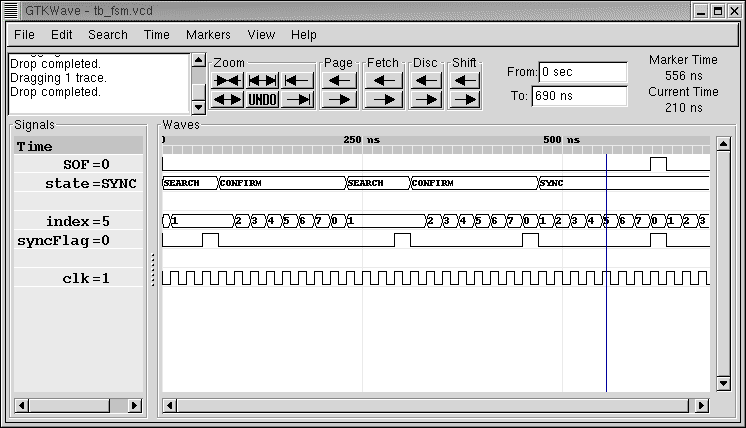
\includegraphics{tbfsm.png}
\fi

MyHDL now has support for waveform viewing. During simulation, signal
changes can be written to a VCD output file.  The VCD file can then be
loaded in a waveform viewer tool.

The user interface of this feature consists of a single function,
\function{trace_sigs()}.  To explain how it works, recall that in
MyHDL, instances are created by calling a function that returns a
sequence of generators. For example:

\begin{verbatim}
tb_fsm = testbench()
\end{verbatim}

To enable VCD tracing, the instance should be created as 
follows instead:

\begin{verbatim}
tb_fsm = trace_sigs(testbench)
\end{verbatim}

As a result, all signals in the hierarchy of the instance will be
traced in an output VCD file called \file{tb_fsm.vcd}. Note that the
argument of \function{trace_sigs()} consists of the uncalled
function. By calling the function under its control,
\function{trace_sigs()} gathers information about the hierarchy and
the signals to be traced.

In addition, \function{trace_sigs()} accepts an arbitrary number of
additional non-keyword and keyword arguments that will be passed
to the function call.





\end{document}
